\newpage
\section{Deployment}\label{sec:03_depl}
% Explain section
This section explains the deployment of the application.
% Requirements
The requirements to run all applications are the following (the versions correspond to the local system of the author):
\begin{itemize}
\item H2\footnote{H2 Database - \url{http://www.h2database.com/}} 2.0.202
\item WildFly\footnote{WildFly - \url{https://www.wildfly.org/}} 20.0.1.Final
\item Java\footnote{OpenJDK - \url{https://openjdk.java.net/}} AdoptOpenJDK-11.0.11+9
\item Apache Tomcat\footnote{Apache Tomcat - \url{https://tomcat.apache.org/}} 9.0.56
\item Apache Maven\footnote{Apache Maven - \url{https://maven.apache.org/}} 3.8.4
\end{itemize}


% Create database
\subsection{H2 Database}\label{sec:03_depl_h2}
% What
As mentioned before, this application uses a local H2 database, that is not integrated into the project itself, but is located somewhere, on the user's computer.

% Start H2
\subsubsection{Start H2}\label{sec:03_depl_h2_start}
At first, it is important to start the H2 service via the terminal. This can be accomplished by executing the command \texttt{\$ java -jar h2*.jar} in the directory \path{$H2/bin}, where \texttt{\$H2} is the path of the H2 database. This process is shown in \Fig{fig:03_depl_h2_h2start}. After executing the command, the H2 console is automatically started in the default web browser, which is needed later.
\begin{figure}[h]
\centering
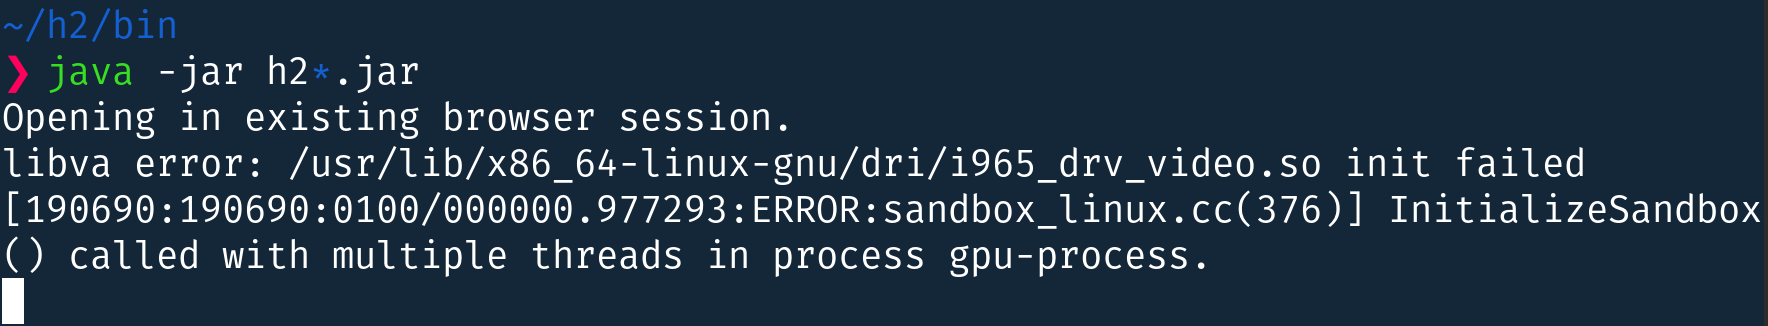
\includegraphics[scale=0.23]{images/03_depl/h2_start}
\caption{Process to start the H2 service}
\label{fig:03_depl_h2_h2start}
\end{figure}

% Create a Database
\subsubsection{Create a Database}\label{sec:03_depl_h2_create}
After the H2 service has been started, it is needed to create a new local database using the shell tool of H2. This process is shown in \Fig{fig:03_depl_createdb_create}, where the command \texttt{\$ java -cp h2-*.jar org.h2.tools.Shell} needs to get executed in the \path{$H2/bin} directory. It is important, that the database is called \textit{accommodations}, the username is \textit{sa}, and the password is \textit{sa} as well.
\begin{figure}[h]
\centering
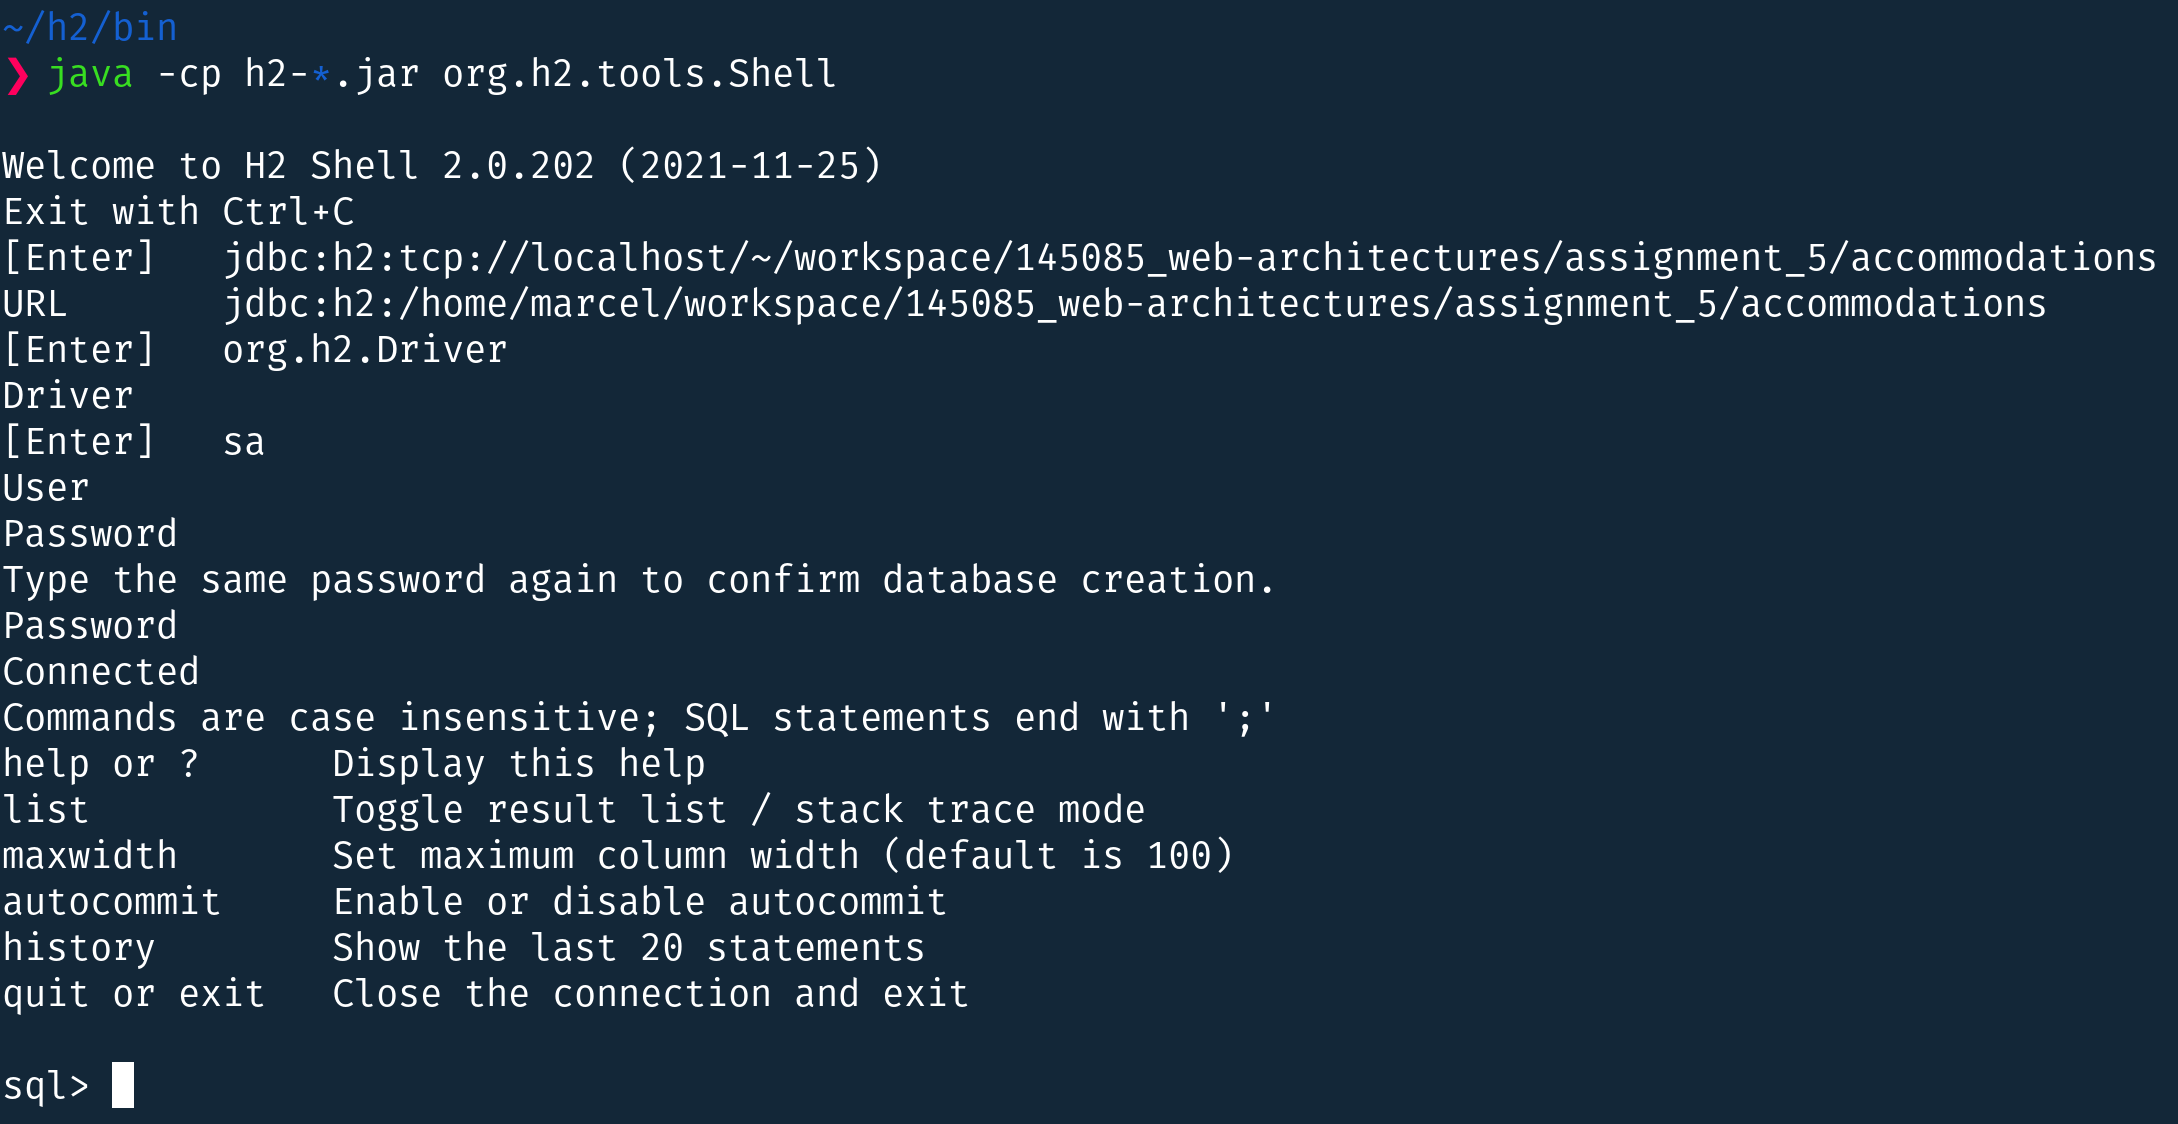
\includegraphics[scale=0.18]{images/03_depl/create-db}
\caption{Process to create a H2 database}
\label{fig:03_depl_createdb_create}
\end{figure}

% Web browser
\subsubsection{Test Database Connection}\label{sec:03_depl_h2_test}
After creating the \textit{accommodations} database, it is possible to test the connection using the H2 console mentioned in \Sec{sec:03_depl_h2_start}.

% How to test
First, it is necessary to fill in the correct information: The JDBC URL in the format \texttt{jdbc:h2:tcp://localhost/PATH\_TO\_DATABASE/accommodations}, and the previously used username and password from \Sec{sec:03_depl_h2_create} (username: \texttt{sa}, password: \texttt{sa}).
% Test
Then, by clicking on \textit{Test Connection}, a status message is shown as illustrated in \Fig{fig:03_depl_createdb_h2test}. If the connection is successful, the database can be used in the application.
\begin{figure}[h]
\centering
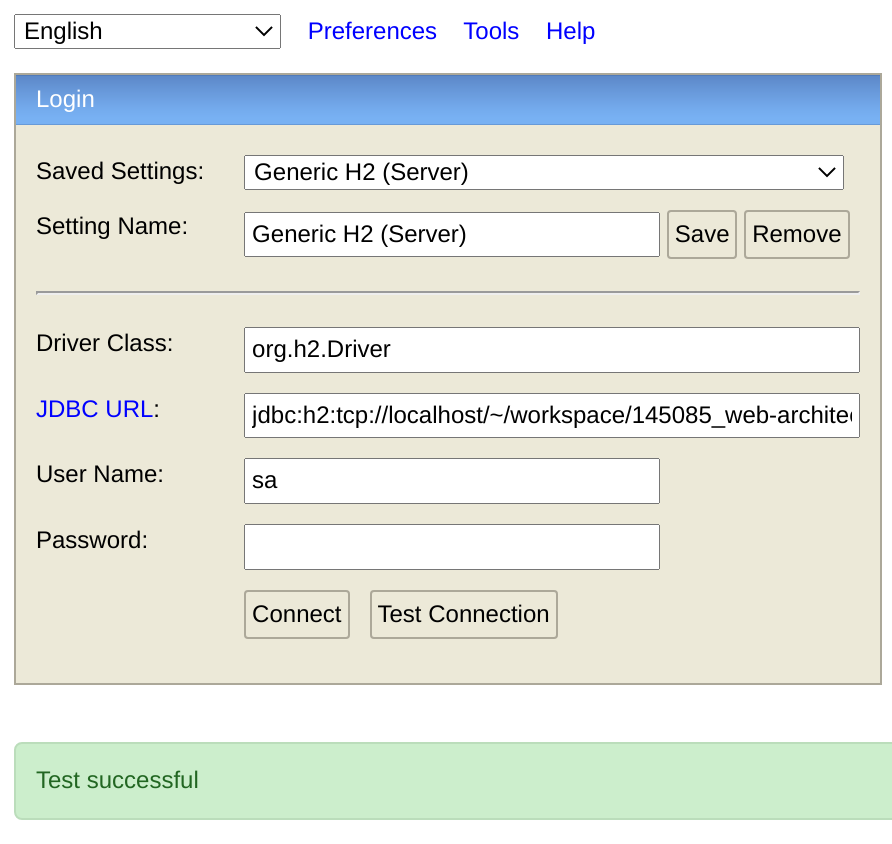
\includegraphics[scale=0.3]{images/03_depl/h2_test}
\caption{Successfull connection test for the H2 database}
\label{fig:03_depl_createdb_h2test}
\end{figure}

\newpage
\subsection{Seeding the Database}\label{sec:03_depl_seeddb}
% What
After the database has been created, it is important to write test data to it using the \textit{DatabaseRoutine} project.

\subsubsection{Set up the DatabaseRoutine application}\label{sec:03_depl_seeddb_setup}
% How
It is important to set the path to the database in the \path{persistance.xml} of the \textit{DatabaseRoutine} project. The \path{persistance.xml} file is located at \path{DatabaseRoutine/src/main/resources/META-INF/persistance.xml}. \Lst{lst:03_depl_seeddb_setup_config} shows a correct configuration. The property \texttt{hibernate.connection.url} has to be set to the URL used in \Sec{sec:03_depl_h2_create}.
\begin{lstlisting}[label=lst:03_depl_seeddb_setup_config, caption=Default data source configuration, language=xml]
...
<persistence-unit name="default">
  <properties>
    <property name="hibernate.connection.url"
              value="jdbc:h2:tcp://localhost/~/workspace/145085_web-architectures/assignment_5/accommodations"/>
  </properties>
</persistence-unit>
...
\end{lstlisting}

\subsubsection{Execute the DatabaseRoutine application}\label{sec:03_depl_seeddb_executeroutine}
% How
To execute the \textit{DatabaseRoutine} application, open the project in IntelliJ, right-click on the \path{DataRoutine.java} file, and select \textit{Run 'DataRoutine.main()'}. Then, the file gets executed and writes dummy data to the database.

% Check
After that, it is possible to check if the data has been written to the database by connecting to the database using the H2 console, introduced in \Sec{sec:03_depl_h2_create}. \Fig{fig:03_depl_seeddb_executeroutine_data} shows the newly created tables in the database.
\begin{figure}[h]
\centering
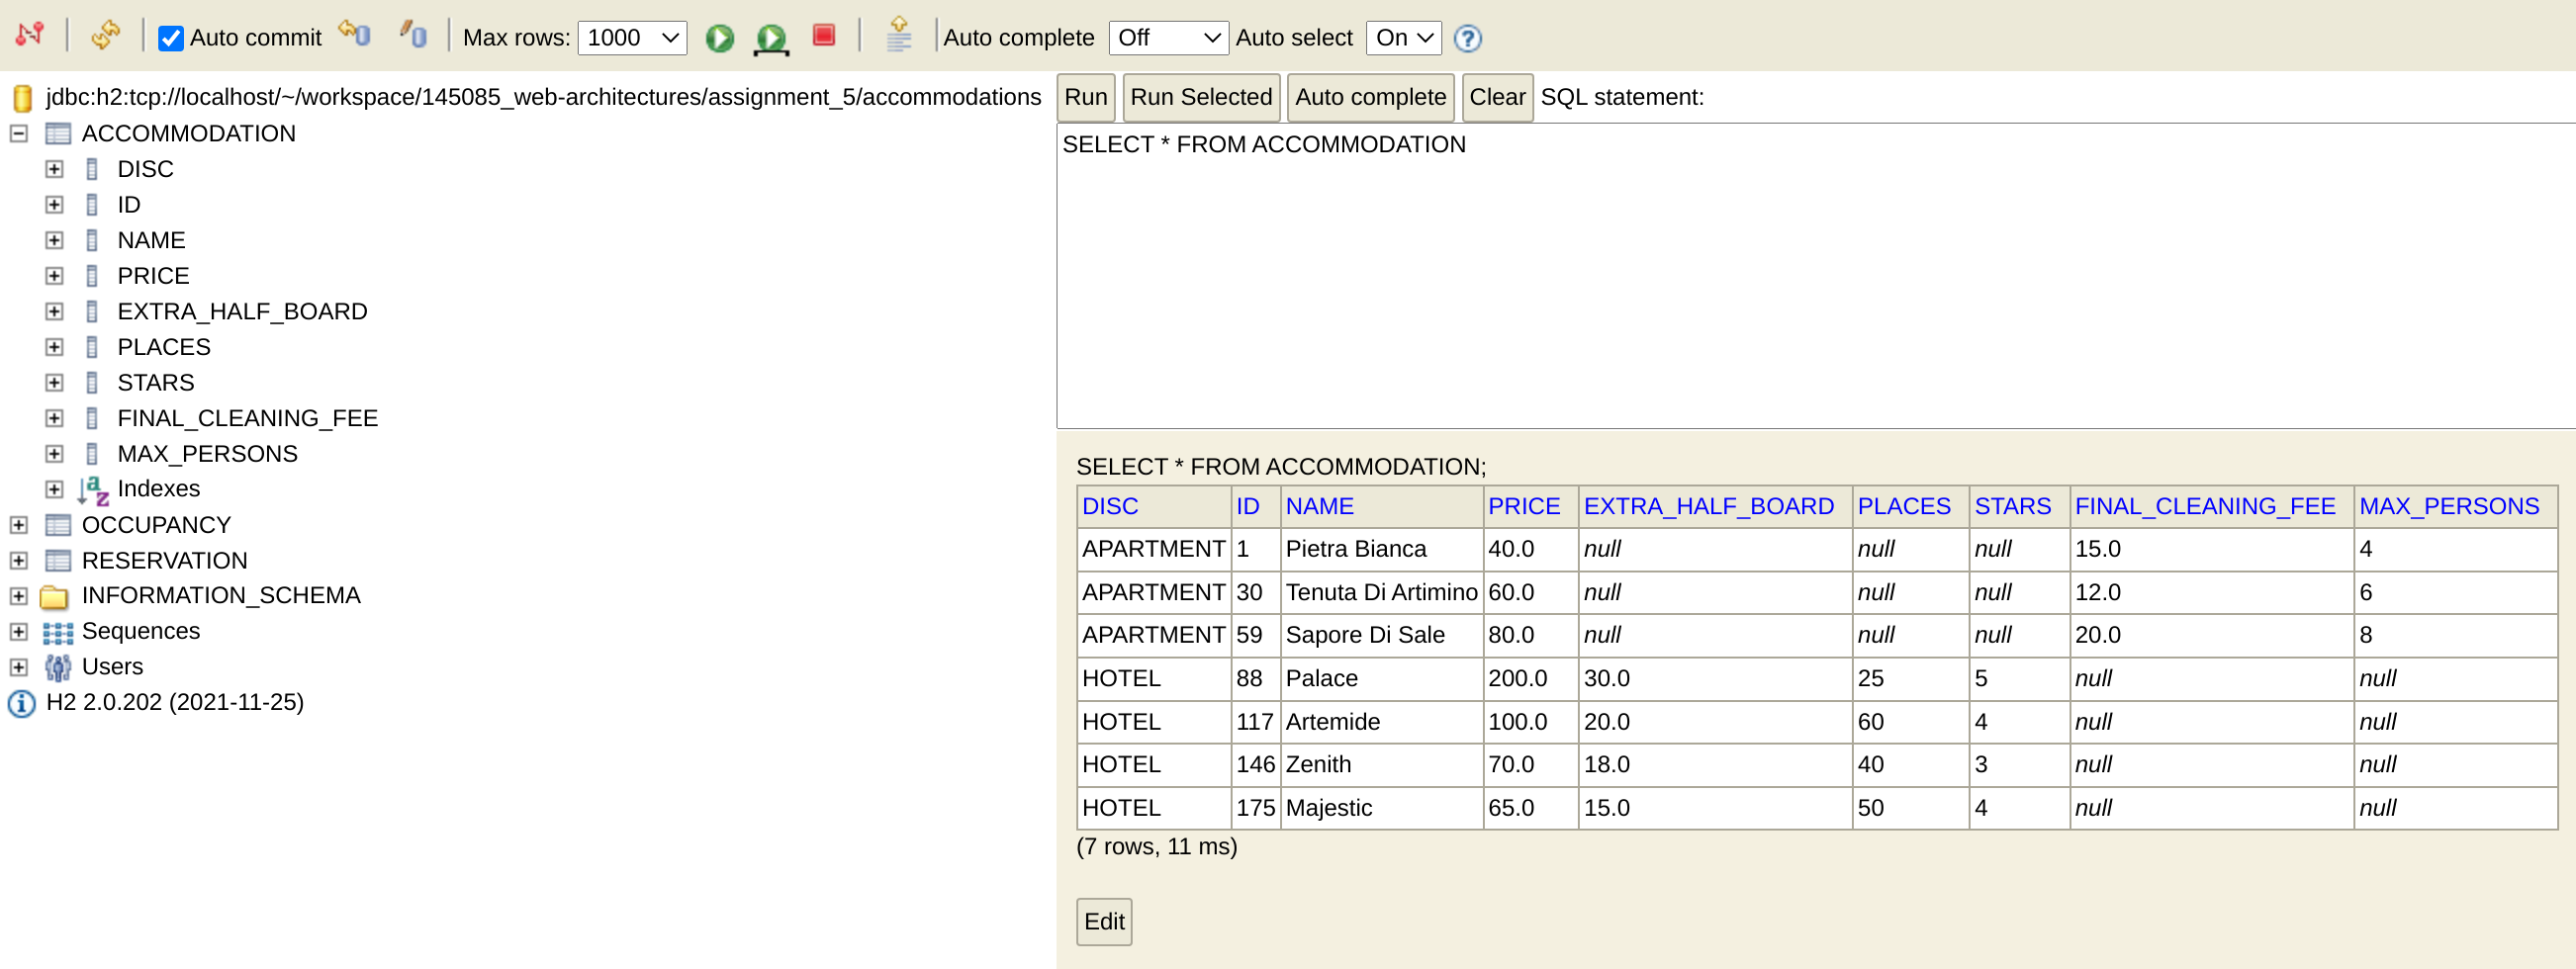
\includegraphics[scale=0.15]{images/03_depl/dummy-data}
\caption{Successfull connection test for the H2 database}
\label{fig:03_depl_seeddb_executeroutine_data}
\end{figure}


\subsection{Setting up WildFly}\label{sec:03_depl_wildfly}
% Set up Wildfly
After the H2 database is created, the EJB`s can be deployed to the WildFly application server.

% H2
It is important to mention, that at this point the H2 database (explained in \Sec{sec:03_depl_h2}) has to be running.

% Set up the datasource
\subsubsection{Add H2 database data source}\label{sec:03_depl_wildfly_datasource}
To give the EJB`s the ability to access the \textit{accommodations} database, it has to be defined as a data source in the configuration file of WildFly. The configuration file is located at \path{$JBOSS_HOME/standalone/configuration/standalone.xml}, where \texttt{\$JBOSS\_HOME} is the path to WildFly. 
% How
\Lst{lst:03_depl_wildfly_datasource_config} shows how the \textit{accommodations} database, created in \Sec{sec:03_depl_h2}, has been added as a data source in WildFly given the name \texttt{AccommodationsDS}.
\begin{lstlisting}[label=lst:03_depl_wildfly_datasource_config, caption=WildFly datasource configuration, language=xml]
...
<subsystem xmlns="urn:jboss:domain:datasources:6.0">
  <datasources>
    <datasource jndi-name="java:jboss/datasources/AccommodationsDS" pool-name="AccommodationsDS" enabled="true" use-java-context="true" statistics-enabled="${wildfly.datasources.statistics-enabled:${wildfly.statistics-enabled:false}}">
      <connection-url>jdbc:h2:tcp://localhost/~/workspace/145085_web-architectures/assignment_5/accommodations;DB_CLOSE_DELAY=-1;DB_CLOSE_ON_EXIT=FALSE</connection-url>
      <driver>h2</driver>
      <security>
        <user-name>sa</user-name>
        <password>sa</password>
      </security>
    </datasource>
    ...
  </datasources>
</subsystem>
...
\end{lstlisting}

% Also to the project
Additionally, this data source has to be added to the \path{persistance.xml} configuration file of the \textit{WebServices} project as well, which is located at \path{WebServices/src/main/resources/META-INF/persistance.xml}.
% Which name
Therefore, a new \textit{jta-data-source} with the value \texttt{java:jboss/datasources/AccommodationsDS} is added to the default \textit{persistence unit}, as shown in \Lst{lst:03_depl_wildfly_datasource_persistance}.

\begin{lstlisting}[label=lst:03_depl_wildfly_datasource_persistance, caption=Default data source configuration, language=xml]
...
<persistence-unit name="default">
  <jta-data-source>java:jboss/datasources/AccommodationsDS</jta-data-source>
  <properties>
    <property name="hibernate.show_sql" value="true"/>
    <property name="hibernate.format_sql" value="true"/>
    <property name="hibernate.use_sql_comments" value="true"/>
  </properties>
</persistence-unit>
...
\end{lstlisting}


% Build EJB jar
\subsubsection{Compile EJB Jar}\label{sec:03_depl_wildfly_jar}
Next, the EJB`s need to be deployed to the WildFly server. Therefore, it is necessary to run the command \texttt{\$ mvn clean package} in the directory of the \textit{WebServices} project, which builds the \texttt{.jar} artifact containing all EJB`s. After that, a new directory called \path{/target} was created in the root folder of the \textit{WebServices} project, where the EJB JAR  \path{marcel-stolin-web-services.jar} is located, which is shown in \Fig{fig:03_depl_wildfly_jar_build}.
\begin{figure}[h]
\centering
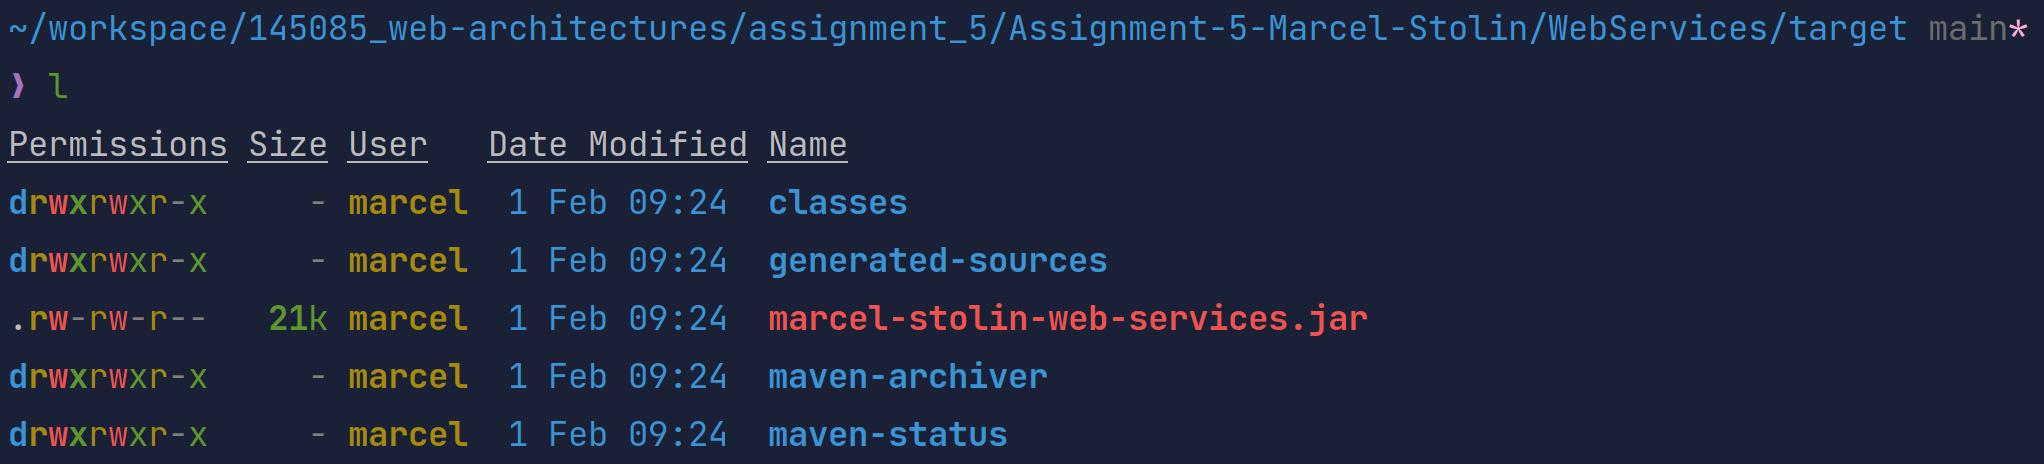
\includegraphics[scale=0.2]{images/03_depl/web-services-artifact}
\caption{Compiled EJB JAR of the \textit{WebServices} project}
\label{fig:03_depl_wildfly_jar_build}
\end{figure}


% Deploy jar
\subsubsection{EJB JAR Deployment}\label{sec:03_depl_wildfly_deploy}
After the \texttt{.jar} artifact has been created, it needs to be copied to the deployment directory of the WildFly server. The artifact can be deployed using the command shown in \Lst{lst:03_depl_wildfly_deploy_command}, where \texttt{\$JBOSS\_HOME} is the path to the local WildFly directory. This command needs to be executed in the project folder of the \textit{WebServices} project, which is shown in \Fig{fig:03_depl_wildfly_deploy_command}.
% Command
\begin{lstlisting}[label=lst:03_depl_wildfly_deploy_command, caption=Command to copy the EJB JAR artifact to the WildFly deployment directory, language=bash]
$ cp target/marcel-stolin-web-services.jar $JBOSS_HOME/standalone/deployments
\end{lstlisting}
% Figure
\begin{figure}[h]
\centering
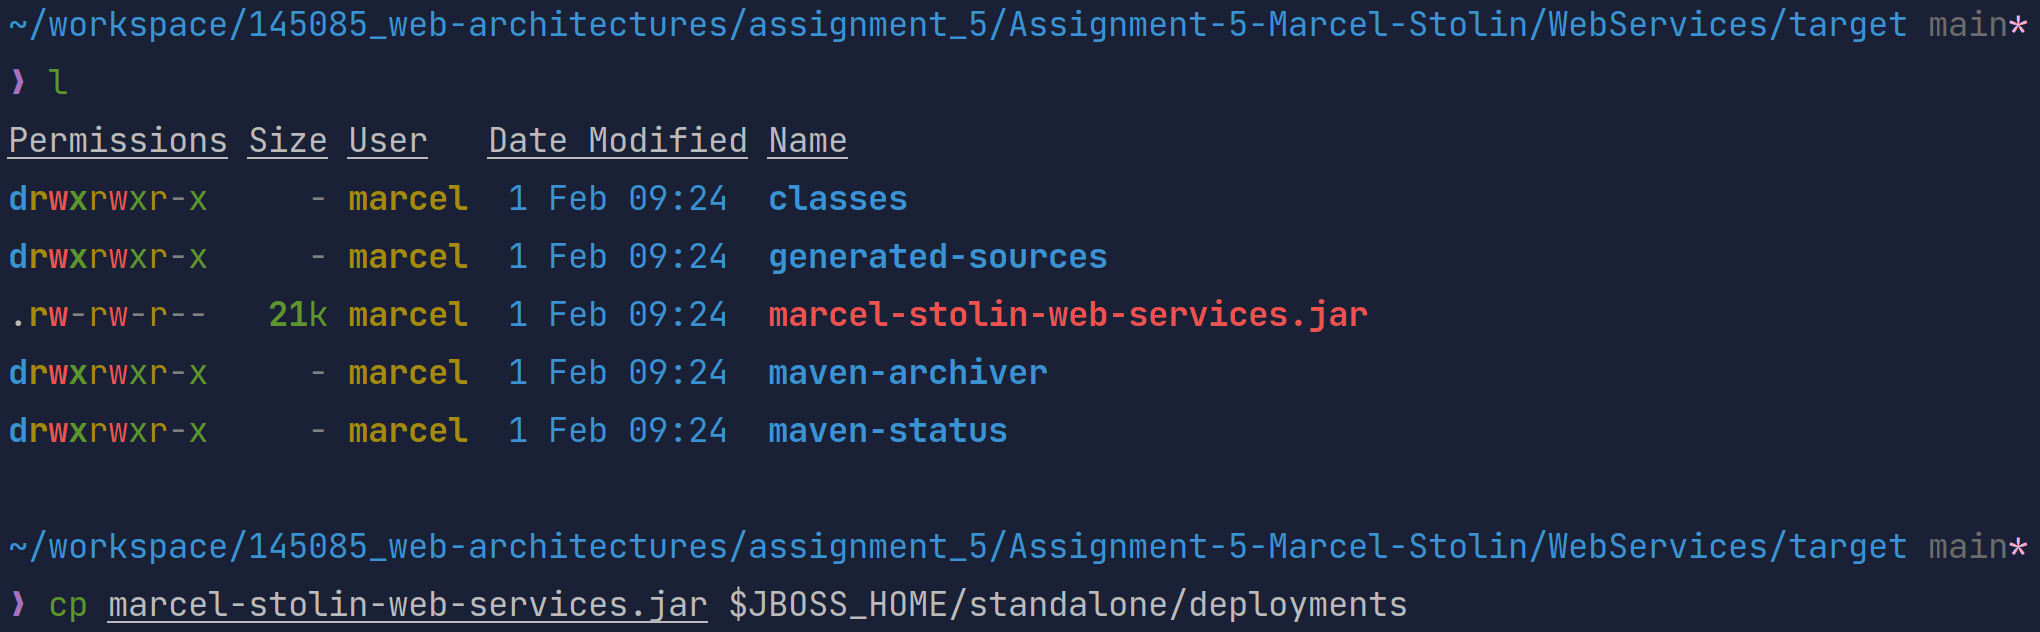
\includegraphics[scale=0.2]{images/03_depl/web-services-deployment}
\caption{Process to deploy the EJB JAR artifact to the WildFly application server}
\label{fig:03_depl_wildfly_deploy_command}
\end{figure}


% Start Wildfly server
\subsubsection{Start Wildfly Application Server}\label{sec:03_depl_wildfly_start}
Finally, the WildFly server can be started using the command \linebreak \texttt{\$ \$JBOSS\_HOME/bin/standalone.sh}. Additionally, the log prints the lookup addresses of both the \textit{AccommodationService} (mentioned in \Sec{sec:02_design_beans_acc}) and the \textit{ReservationService} (mentioned in \Sec{sec:02_design_beans_reservation}), which is illustrated in \Fig{fig:03_depl_wildfly_start_addresses}.
\begin{figure}[h]
\centering
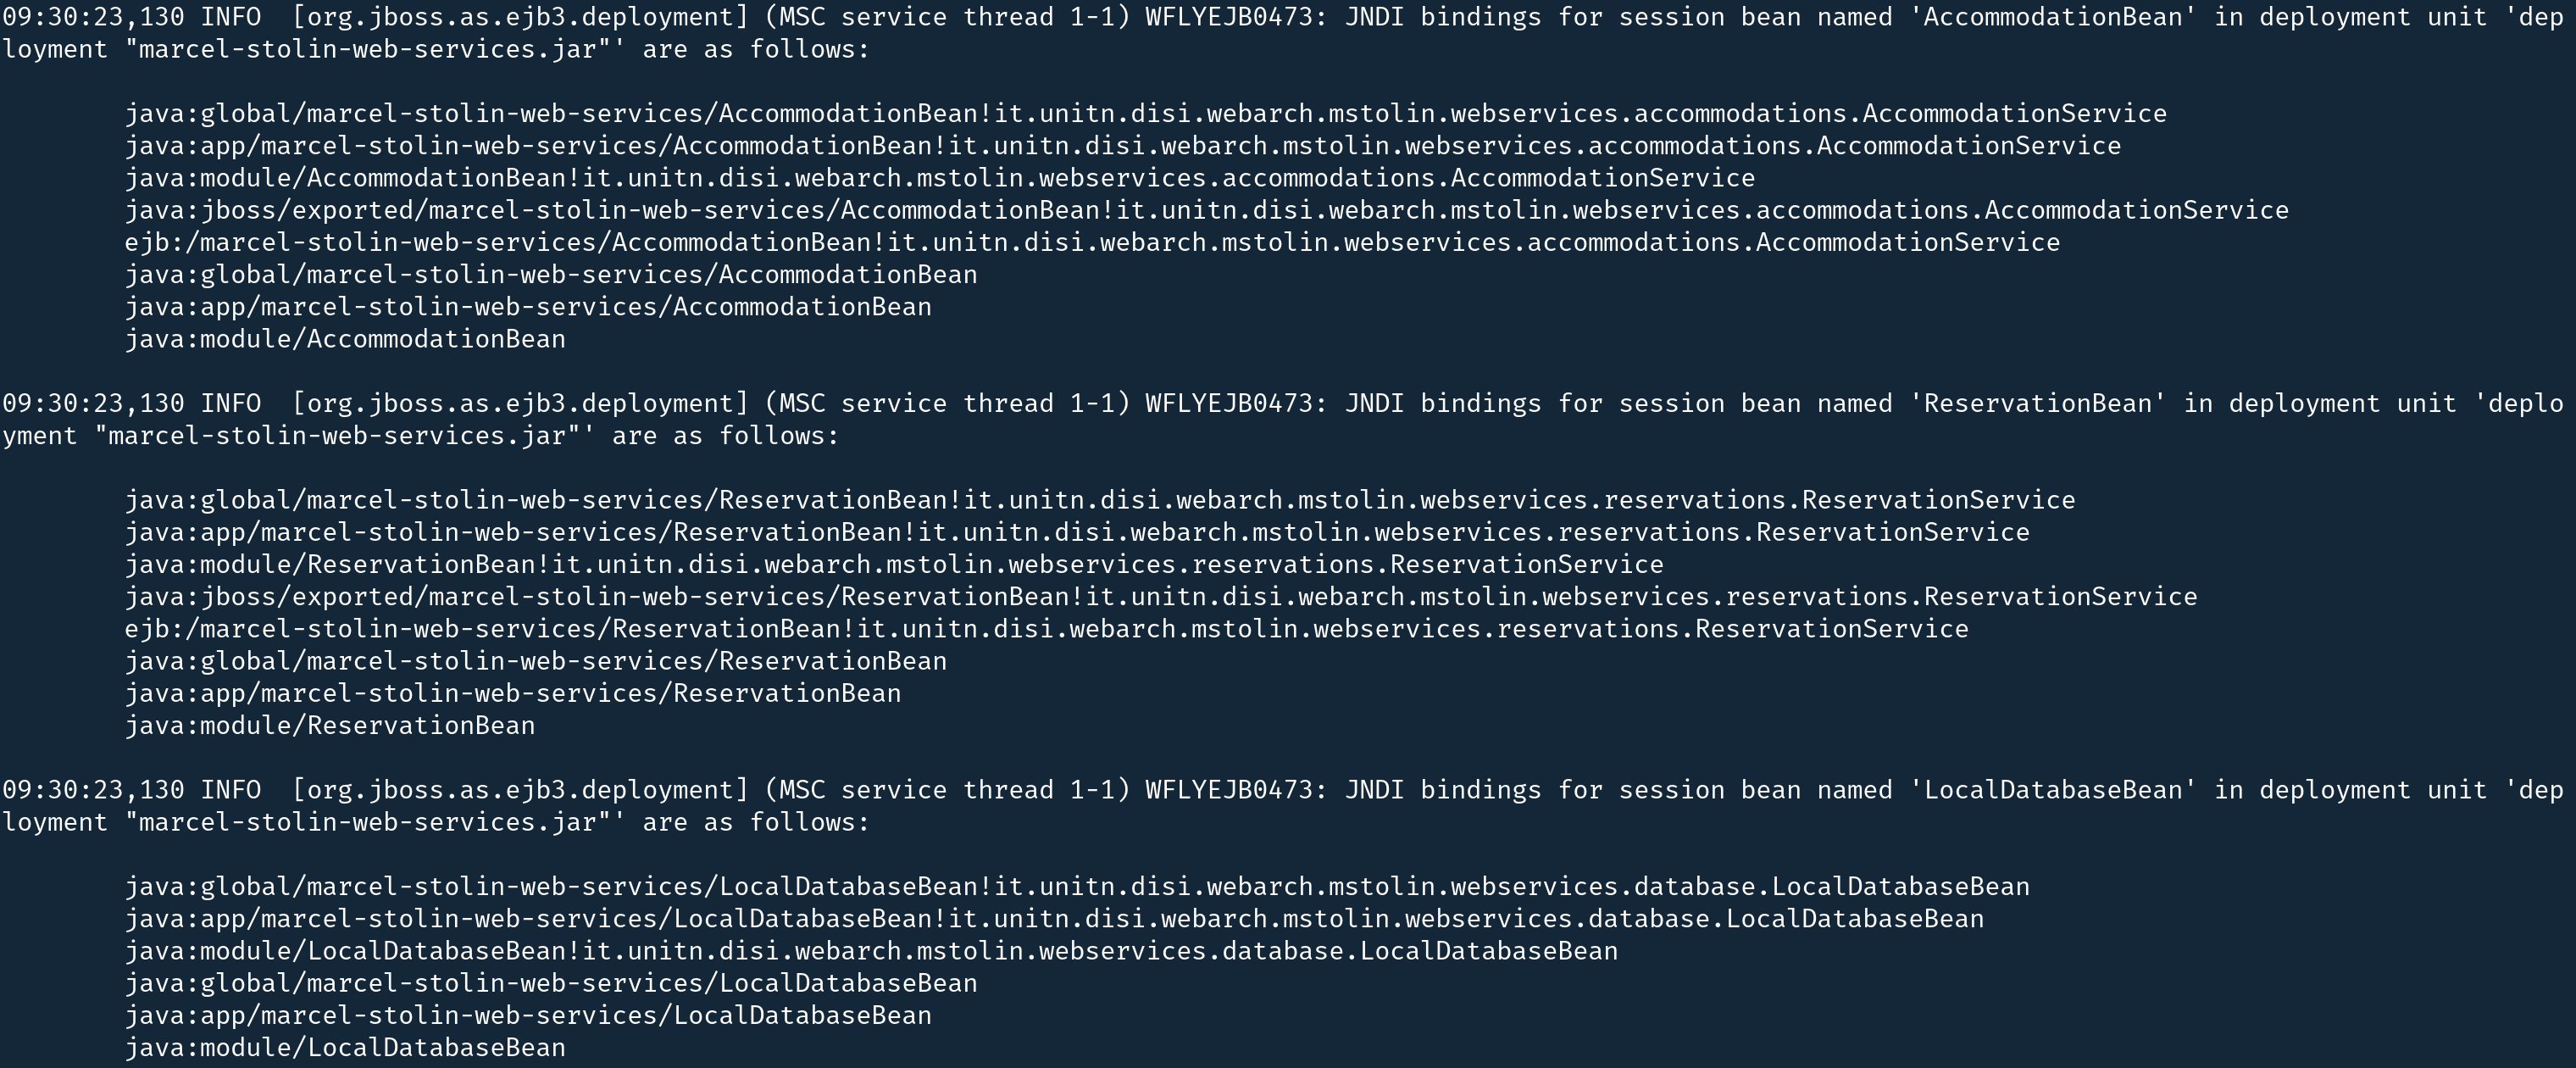
\includegraphics[scale=0.13]{images/03_depl/deployed-beans}
\caption{WildFly application server Log}
\label{fig:03_depl_wildfly_start_addresses}
\end{figure}


\subsection{Starting the Web Application}\label{sec:03_depl_webapp}
% Important things
After the database has been created successfully, and the EJB`s have been deployed successfully, the web application can be deployed to Apache Tomcat.

% Different port
One problem is, that WildFly already uses port 8080, and Apache Tomcat uses port 8080 by default as well. Therefore, Apache Tomcat has to be configured to use port 8000 instead. 

% Intellij
For this project, the IntelliJ IDEA is used to start and deploy the \textit{WebApp} project on Apache Tomcat. Therefore, it is necessary to create a \textit{Run Configuration} for Apache Tomcat for the \textit{WebApp} project.

% Server
\subsubsection{Server Settings}
The \textit{Server} settings for IntelliJ are shown in \Fig{fig:03_depl_webapp_intellij_config1}. It is important, that the URL is set to \url{http://localhost:8000/marcel-stolin-web-app/} and the HTTP port, at \textit{Tomcat Server Settings},  is set to 8000. In addition, under \textit{Before launch} it is important to build the \textit{WebApp:war exploded} artifact.
\begin{figure}[h]
\centering
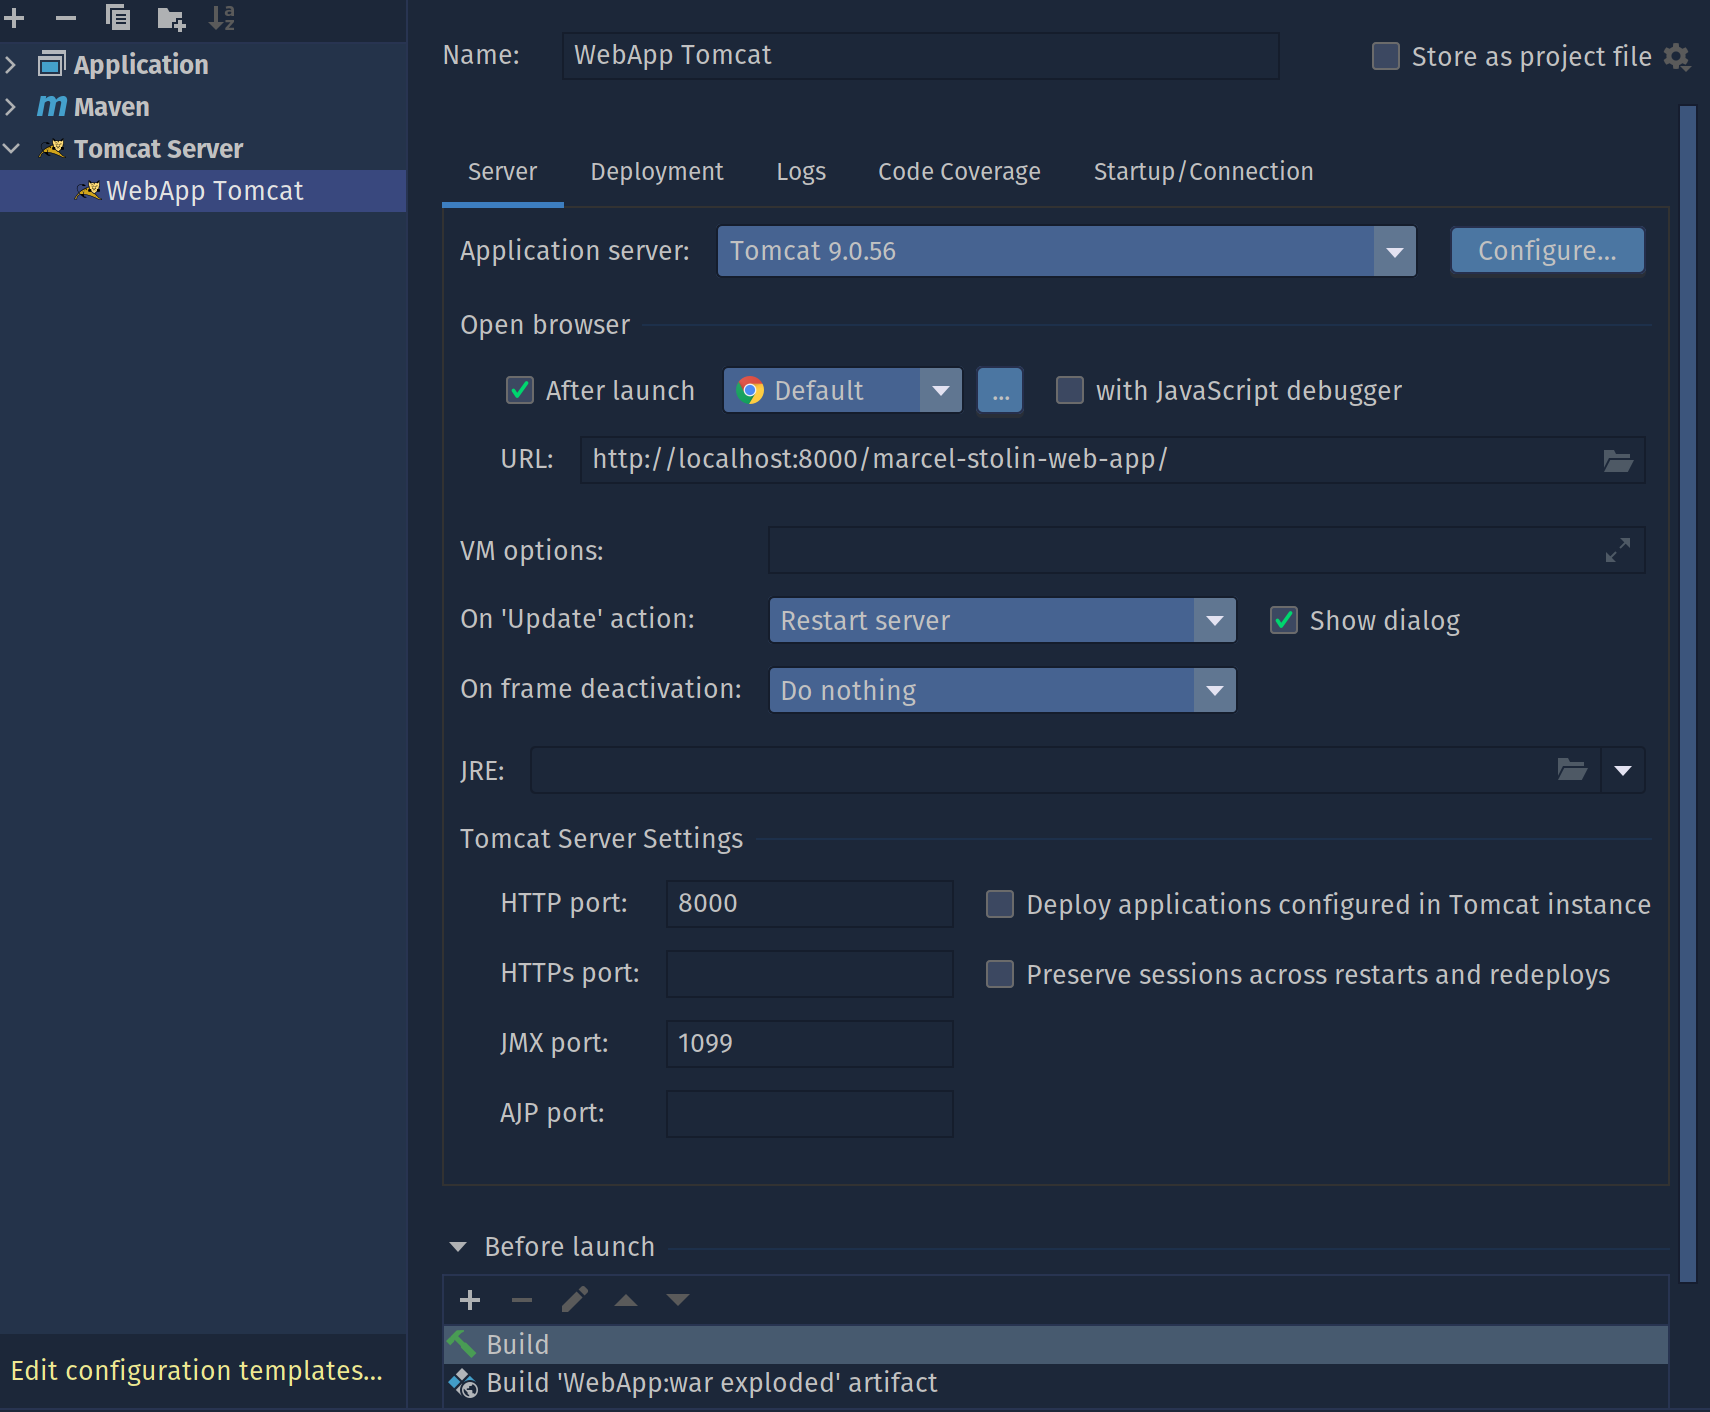
\includegraphics[scale=0.2]{images/03_depl/tomcat-config-1}
\caption{IntelliJ Tomcat Configuration Server Settings}
\label{fig:03_depl_webapp_intellij_config1}
\end{figure}

% Deployment
\subsubsection{Deployment Settings}
\Fig{fig:03_depl_webapp_intellij_config2} shows the settings for the \textit{Deployment} section. It is necessary to deploy the \textit{WebApp:war exploded} artifact on server startup. Additionally, the \textit{Application Context} needs to be set to \texttt{marcel-stolin-web-app}.
\begin{figure}[h]
\centering
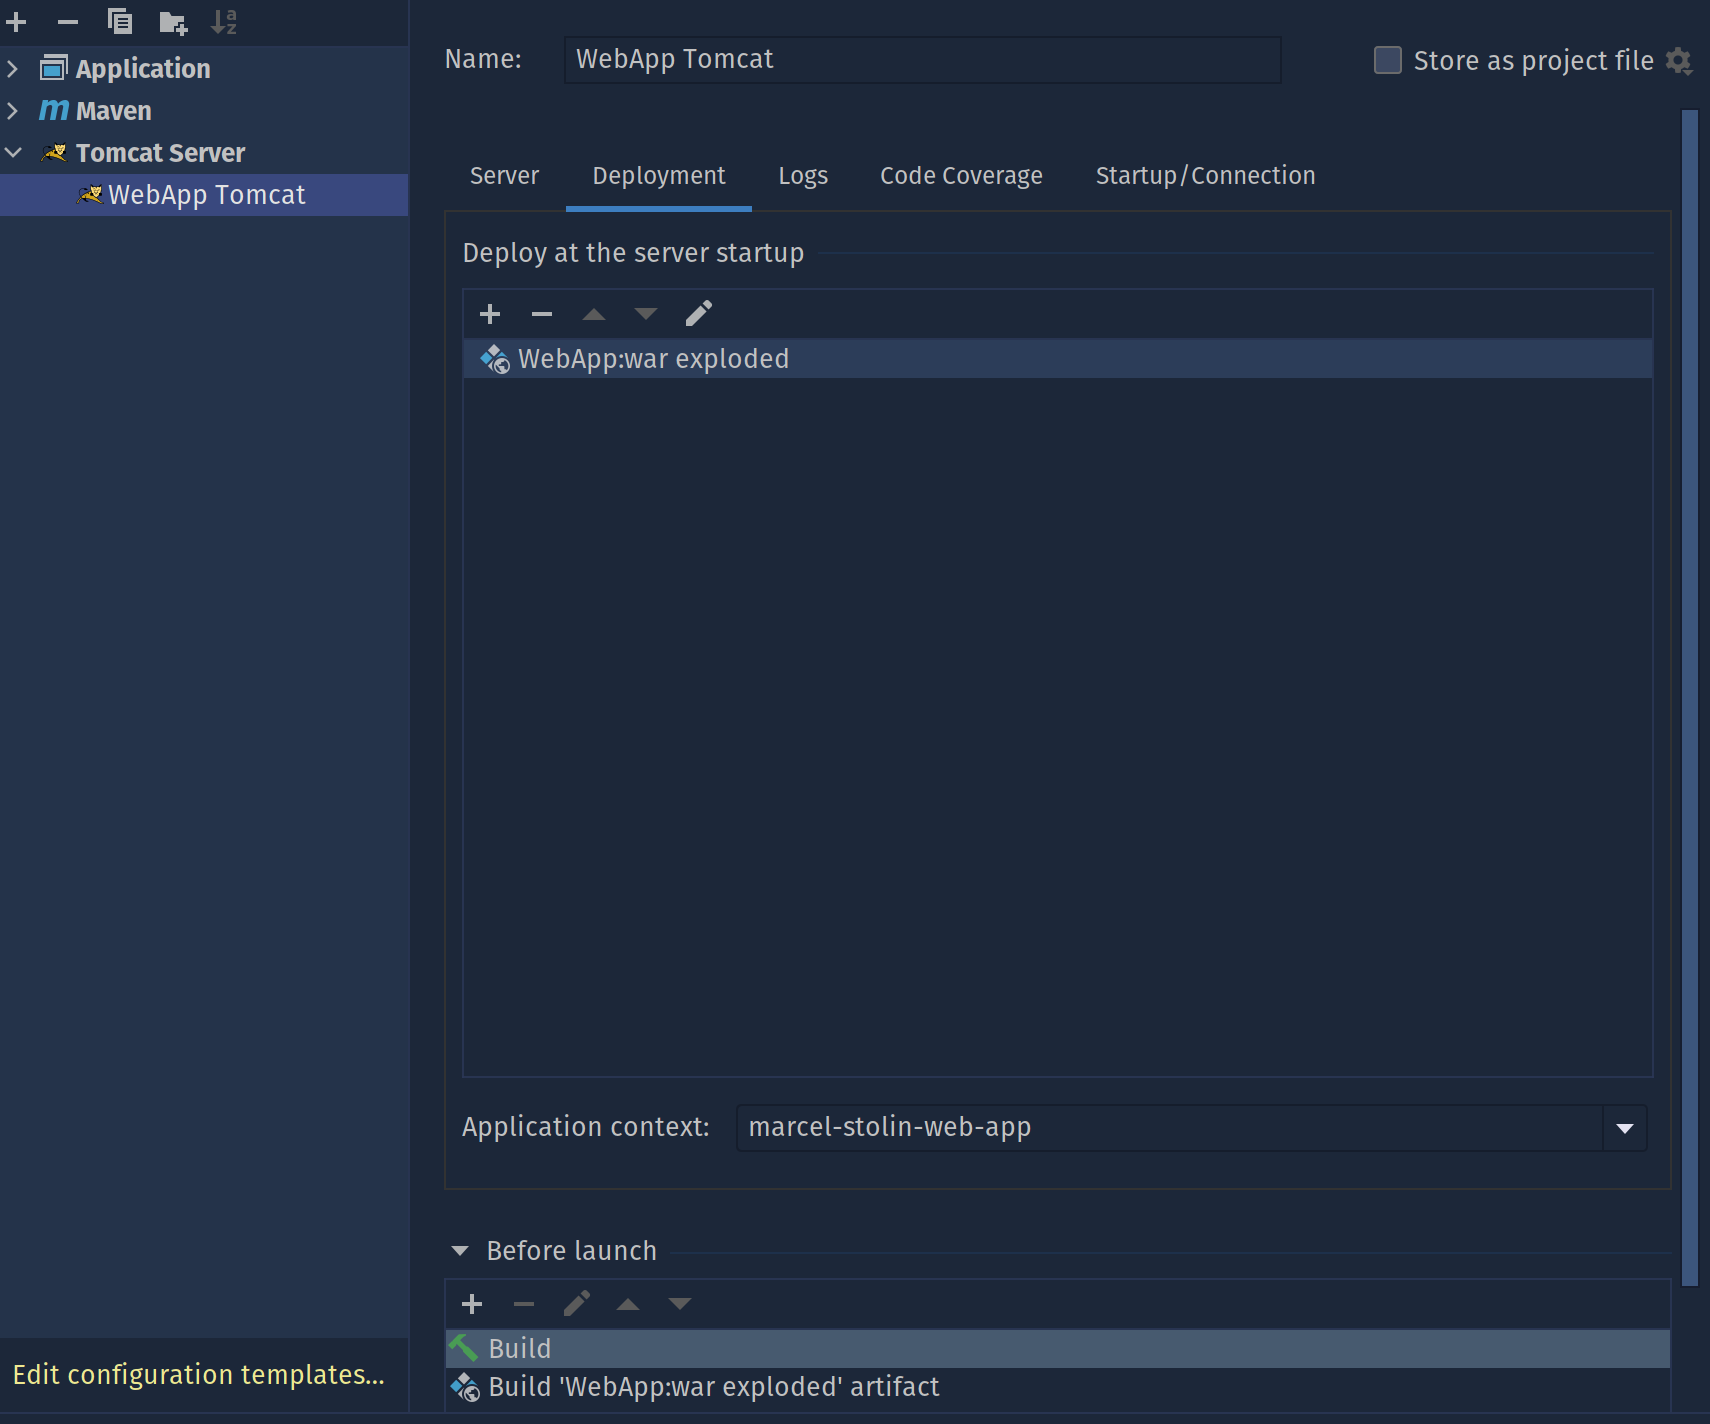
\includegraphics[scale=0.2]{images/03_depl/tomcat-config-2}
\caption{IntelliJ Tomcat Configuration Deployment Settings}
\label{fig:03_depl_webapp_intellij_config2}
\end{figure}

% Start server
\subsubsection{Starting the Application}
By running the Apache Tomcat \textit{Run Configuration}, the web application is available at \url{http://localhost:8000/marcel-stolin-web-app/}.
